\section{Introduction}

Event extraction is the task of finding specific events and then extracting structured knowledge of the events from
unstructured data such as news articles, tweets, or blogs. It is an important technique that underpins many text mining
applications such as news recommendation and information filtering.
The goal of event extraction is to discover structured information about an event occurrence like ``\emph{who did what to whom,
when, where through what methods, and why}"~\cite{Piskorski2013}. A concrete example of event extraction is
given in Figure 1. Given a text
document, an event extraction system should be able to identify all the relevant entities and their relationships.


\begin{quote}
S1: 俄罗斯石油公司 \hspace{0.3cm}收购 \hspace{0.3cm}尤甘斯克 \hspace{0.3cm}付出 \hspace{0.2cm}了 \hspace{0.2cm}仅 \hspace{0.3cm}93.5
\hspace{0.3cm}亿 \hspace{0.3cm}美元。

\hspace{0.52cm} Rosneft acquired Yugansk, paying only 9.35 billion dollars.
\end{quote}

Finding a set of high-quality features, i.e. feature engineering, is key to event extraction.
Most current approaches rely on hand-crafted features to build multi-class classifiers to perform various
event-extraction-related tasks~\cite{ahn2006stages,chen2009language,li2012employing,chen2012joint}. The
features used in prior work can be divided into two categories: \emph{lexical features} and \emph{sentence-level features}, where the
former are designed to capture the local information of words, such as part-of-speech tags or word lemma, while the latter are used to
characterize the topic of the whole sentence. The challenge of finding useful
features is that the space of possible features is vast, while their effect depends on various factors: the natural language, the structure of the data, and the application domain.

\begin{figure}
\centering
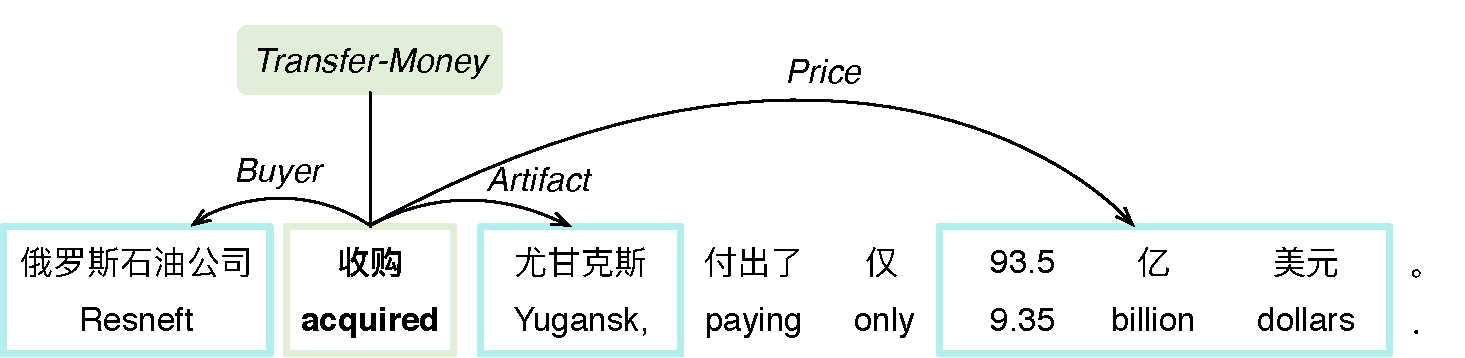
\includegraphics[width=.9\textwidth]{example.pdf}
\caption{An example of Chinese event extraction for S1, where English translations are provided besides the Chinese words. The example sentence has one \emph{Transfer-Money} event mention triggered by \textit{收购 (acquired)}, which have three arguments, \textit{俄罗斯石油公司 (Rosneft)} as the \emph{Transfer-Money} event's \textit{Buyer}, \textit{尤甘斯克 (Yugansk)}  as its \textit{Artifact}, and \textit{93.5 亿美元 (9.35 billion dollars)} as its \textit{Price}.}
\label{exfigure}
\end{figure}


Despite much progress has been made in English event extraction, building an effective Chinese event extraction system remains a challenge.
There have been efforts to solve this problem using hand-crafted feature templates building upon specific natural language processing (NLP)
tools, such as POS tagging\FIXME{~\cite{}}, syntactic parsing\FIXME{~\cite{}}, semantic role labeling\FIXME{~\cite{}}, and so on. While it
is possible to manually design a set of task-specific feature templates, current approaches require extensive human involvement and are
tightly couple to the information provided by specific NLP tools. This means that when we target a new  language,  where limited tools or
resources are available, despite of the time-consuming process of feature engineering, the system will be heavily affected by the
performance of existing NLP tools for that new language. Unfortunately, most low-resourced languages have far-from-perfect performances
even in their fundamental semantic or syntactic analysis, e.g., Chinese syntactic parsing performance is around 5\% lower than that of
English in newswire, which leads to significant performance drop in downstream applications. Therefore, it is essential to have a technique
that can automatically discover lexical and sentence-level feature representations for event extraction in a low-resourced language, with
little human involvement and does not heavily depend on specific NLP tools.

In this paper, we propose to utilize neural networks to alleviate the burden of feature
engineering for Chinese event extraction. To do so, we develop a convolution bidirectional long short-term memory
(\LSTM) network (\CBiLSTM) to automatically learn lexical and sentence level feature representations without extensive human
involvement. We achieve this by first constructing a bidirectional \LSTM to encode the entire sentence into
sentence-level features without performing dependency parsing or semantic role labeling (\SRL). % -- which require inputs from human experts~\cite{}.
We then take advantage of a convolutional neural network to capture salient local features
to semantically characterize event occurrences, %recognize and classify how the event is triggered,
without relying on part-of-speech (\POS) tagging or named entity
recognition (\NER). %This allows us to build a system to automatically extract local lexical features.
To address the word segmentation issue which is a fundamental but challenging step for Chinese language processing, we employ a conditional
random field (\CRF) layer to automatically learn sentence-level labeling constraints and jointly decode the best labeling sequence for the
whole sentence.

Putting together these techniques, we are able to build a powerful
system for Chinese event extraction. As we show, our approach can
automatically learn feature representations that lead to the same level of performance compared to hand-tuned features selected by %independent
human experts. This is truly remarkable when one considers that our approach is given no prior knowledge of
the syntax or semantics of the target language. %\FIXME{Check the last sentence.}

We evaluate our approach on the ACE 2005 Chinese event extraction corpus which consists of 8 event types and 33 subtypes.
We compare our approach against a set of well-established traditional feature-based models available for this heavily-studied data set.
The experimental results show that our automatic approach can effectively learn both local semantic and sentence level
representations for event extraction and deliver state-of-the-art performance, when compared to
the hand-tuned features developed by human experts.

%The technical contributions of this work can be summarized as follows. It is the first to
%\begin{itemize}
%\item blabla
%\item blabla
%\item blabla
%\end{itemize}

The rest of this paper is organized as follows. Section~\ref{background} explains the terminologies and defines the
scope of the work. Section~\ref{related} discusses related Chinese event extraction systems. Section ~\ref{trigger} and
Section~\ref{argument} present the neural network models applied to trigger labeling and argument labeling.
Section~\ref{experiment} presents the experimental results and analyses. We conclude our work in
Section~\ref{conclude}.
